% Generated by paper/scripts/generate_tables.py; do not edit by hand.
\begin{figure}[!htbp]
\centering
\resizebox{0.92\linewidth}{!}{%
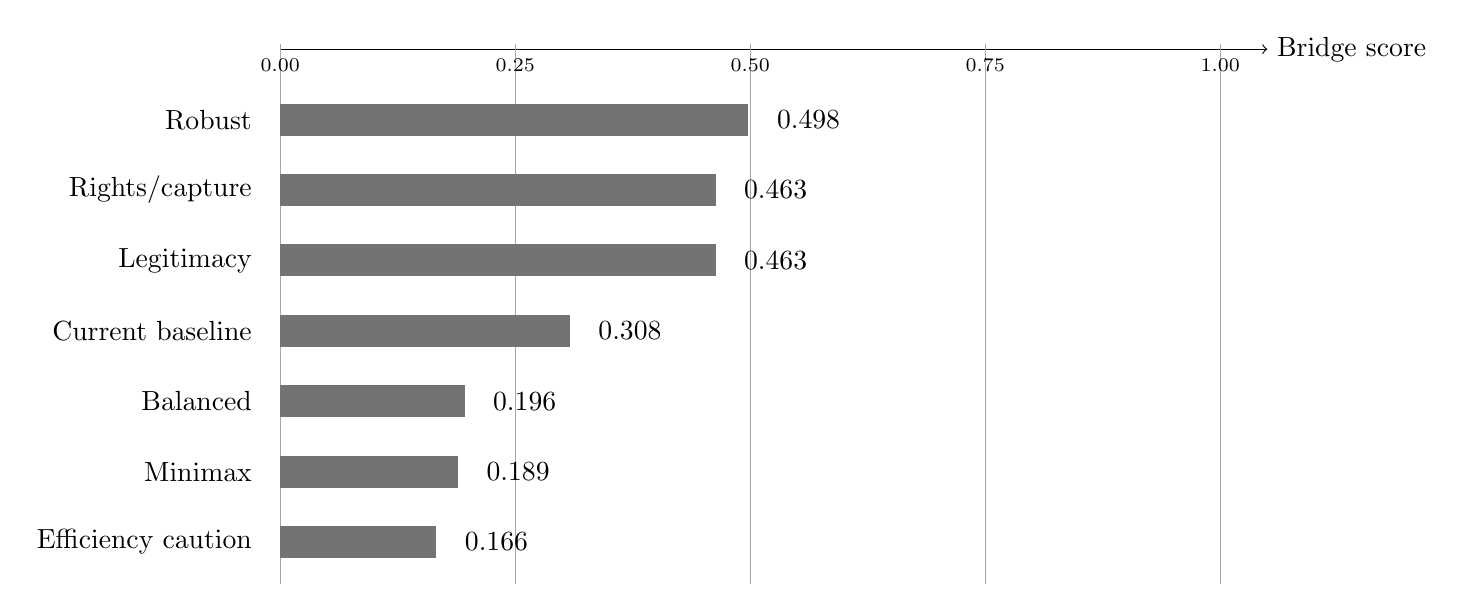
\begin{tikzpicture}[x=4.7in,y=0.80in]
\draw[->] (0,0) -- (1.05,0) node[anchor=west] {Bridge score};
\foreach \x/\lab in {0/0.00,0.25/0.25,0.50/0.50,0.75/0.75,1.00/1.00} {
  \draw[black!35] (\x,0.03) -- (\x,-3.34);
  \node[anchor=north] at (\x,0) {\scriptsize \lab};
}
\node[anchor=east] at (-0.02,-0.44) {Robust};
\fill[black!55] (0,-0.54) rectangle (0.498,-0.34);
\node[anchor=west] at (0.518,-0.44) {0.498};
\node[anchor=east] at (-0.02,-0.88) {Rights/capture};
\fill[black!55] (0,-0.98) rectangle (0.463,-0.78);
\node[anchor=west] at (0.483,-0.88) {0.463};
\node[anchor=east] at (-0.02,-1.32) {Legitimacy};
\fill[black!55] (0,-1.42) rectangle (0.463,-1.22);
\node[anchor=west] at (0.483,-1.32) {0.463};
\node[anchor=east] at (-0.02,-1.76) {Current baseline};
\fill[black!55] (0,-1.86) rectangle (0.308,-1.66);
\node[anchor=west] at (0.328,-1.76) {0.308};
\node[anchor=east] at (-0.02,-2.20) {Balanced};
\fill[black!55] (0,-2.30) rectangle (0.196,-2.10);
\node[anchor=west] at (0.216,-2.20) {0.196};
\node[anchor=east] at (-0.02,-2.64) {Minimax};
\fill[black!55] (0,-2.74) rectangle (0.189,-2.54);
\node[anchor=west] at (0.209,-2.64) {0.189};
\node[anchor=east] at (-0.02,-3.08) {Efficiency caution};
\fill[black!55] (0,-3.18) rectangle (0.166,-2.98);
\node[anchor=west] at (0.186,-3.08) {0.166};
\end{tikzpicture}
}
\caption{High-capture bridge scores across the focused bridge cases.}
\end{figure}
